\documentclass[11pt,a4paper]{article}

% Font: keep Latin Modern (serif) - user preference
\usepackage[utf8]{inputenc}
\usepackage[T1]{fontenc}
\usepackage[english]{babel}
\usepackage{lmodern}
\usepackage{microtype}

% Layout
\usepackage[margin=2.5cm, top=2.5cm, bottom=2.5cm]{geometry}
\usepackage{setspace}
\setstretch{1.12}
\setlength{\parskip}{4pt}
\setlength{\parindent}{0pt}

% Float / page-break control
\widowpenalty=10000
\clubpenalty=10000
\displaywidowpenalty=10000
\renewcommand{\topfraction}{0.9}
\renewcommand{\bottomfraction}{0.9}
\renewcommand{\textfraction}{0.07}
\renewcommand{\floatpagefraction}{0.85}
\setcounter{topnumber}{3}
\setcounter{bottomnumber}{3}
\setcounter{totalnumber}{5}

% Packages
\usepackage{graphicx}
\usepackage{booktabs}
\usepackage{tabularx}
\usepackage{amsmath,amssymb}
\usepackage{xcolor}
\usepackage{float}
\usepackage{caption}
\usepackage{subcaption}
\usepackage{placeins}     % \FloatBarrier to keep floats within sections
\usepackage{enumitem}
\setlist{itemsep=2pt, parsep=0pt, leftmargin=1.5em, topsep=4pt}
\usepackage[round,authoryear]{natbib}
\usepackage[hidelinks,colorlinks=true,linkcolor=black,citecolor=blue!60!black,urlcolor=blue!60!black]{hyperref}
\usepackage{cleveref}

% Figures path: section files can use \includegraphics{configA_*.png} directly
\graphicspath{{figures/}}

% Section formatting (TM style: numbered with trailing period)
\usepackage{titlesec}
\titlespacing*{\section}{0pt}{14pt}{6pt}
\titlespacing*{\subsection}{0pt}{10pt}{3pt}
\titlespacing*{\subsubsection}{0pt}{8pt}{2pt}
\titleformat{\section}{\Large\bfseries}{\thesection.}{0.5em}{}
\titleformat{\subsection}{\large\bfseries}{\thesubsection}{0.5em}{}
\titleformat{\subsubsection}{\normalsize\bfseries}{\thesubsubsection}{0.5em}{}

% Captions: small, tight, bold label, below figures and tables
\captionsetup{font=small, skip=4pt, labelfont=bf, justification=centering,
              singlelinecheck=true}
\captionsetup[table]{position=below, skip=4pt}
\captionsetup[figure]{position=below, skip=4pt}

% Header / footer: empty header, centred page number
\usepackage{fancyhdr}
\pagestyle{fancy}
\fancyhf{}
\fancyfoot[C]{\thepage}
\renewcommand{\headrulewidth}{0pt}
\fancypagestyle{plain}{\fancyhf{}\fancyfoot[C]{\thepage}\renewcommand{\headrulewidth}{0pt}}

\begin{document}

% Title page
\begin{titlepage}
    \centering
    \vspace*{2.5cm}

    {\Huge\bfseries Reinforcement Learning\\[8pt] for Sepsis Treatment in the ICU\par}

    \vspace{1.2cm}

    {\Large Tabular and Deep Methods\\[4pt] on the ICU-Sepsis-v2 Benchmark\par}

    \vspace{2.8cm}

    {\large
    \begin{tabular}{c}
        \textbf{Group X}\\[12pt]
        Samuel Braun, 20250487\\
        Paul Harnos, 20250487\\
        Author 3, Student ID\\
        Author 4, Student ID\\
        Author 5, Student ID\\
    \end{tabular}
    \par}

    \vspace{2cm}

    {\large Reinforcement Learning -- 2025/2026\par}

    \vfill

    {\large NOVA Information Management School\par}
    {\small June 2026\par}
\end{titlepage}

% Table of contents
\pagenumbering{roman}
\tableofcontents
\clearpage
\pagenumbering{arabic}
\setcounter{page}{1}

% Abstract on its own opening page
\begin{abstract}\noindent
This project develops and compares reinforcement learning agents on the ICU-Sepsis-v2 benchmark, a Markov Decision Process fitted to MIMIC-III patient trajectories. Two configurations expose the same underlying MDP through different observation models: a discrete 716-state index amenable to tabular methods, and a 47-dimensional continuous physiological vector wrapped in three clinical-reality failure modes that forces function approximation. Value Iteration achieves 78.8\% survival under fixed cohort difficulty (SOFA bias 5.0, $\lambda = 0.02$ intensity penalty). Q-Learning and SARSA reach 76.1\% and 74.3\% respectively, both indistinguishable at an optimality ratio of 0.877 across three training seeds. The function-approximation agents perform sharply worse: Linear Q-learning collapses to a degenerate single-action policy at 66.6\% survival, while DQN reaches 67.4\% with a clinically sensible SOFA-responsive policy. A bridge experiment deploys the optimal tabular policy on the clinical environment, isolating the irreducible 0.3 percentage-point cost of the acute-event wrapper from the 11.1 percentage-point cost of learning from raw observations. A creative extension introduces risk-sensitive Q-Learning via a Lagrangian death penalty $\beta$, which raises survival from 72.5\% at $\beta=0$ to 76.6\% at $\beta=2$ while leaving the 5\%-quantile of returns unchanged. The findings argue that algorithm class should follow the observation model, and that the standard expected-return objective hides a meaningful tension between treatment intensity and survival in this MDP.
\end{abstract}

\section{Introduction}
\label{sec:intro}

Sepsis is one of the leading causes of death in intensive care units worldwide, accounting for millions of fatalities each year. Treatment is high-stakes and sequential: the clinician decides how much vasopressor to administer to stabilise blood pressure and how much intravenous fluid to give to maintain circulation, then observes the patient's response and decides again. Too little intervention and the patient deteriorates; too much and the treatment itself causes harm. The choice is repeated every few hours over a stay that may last days.

Reinforcement learning is a natural framing for this problem. The clinician's decision rule is a policy, the patient's evolving physiology is a state, and survival is a delayed terminal reward. An RL agent trained on historical trajectories could in principle uncover treatment strategies that improve outcomes beyond what clinical guidelines alone produce. The same framing also makes the limitations visible: the dataset is observational, the action space is coarse, and any policy learned in a simulator may not transfer to bedside care without further validation.

\subsection{The benchmark}

ICU-Sepsis-v2~\citep{choudhary2024icusepsis} is a gymnasium environment fitted to the MIMIC-III critical care database~\citep{johnson2016mimic} using the AI Clinician methodology of \citet{komorowski2018ai}. The MDP has 716 states (714 clinical, 2 terminal corresponding to survival and death) and 25 actions, decomposed as 5 vasopressor levels by 5 IV fluid levels. The reward is sparse: $+1$ on survival, $0$ on death, $0$ at all intermediate steps. Episodes terminate when the patient outcome is realised, with discount factor $\gamma = 1$.

This project applies two configurations of the same MDP. \emph{Configuration A} exposes the discrete state index directly. Tabular RL is feasible at that scale, and the agent has access to the full transition tensor $P$ and reward matrix $R$. \emph{Configuration B} replaces the state index with the 47-dimensional continuous physiological feature vector that produced the state clustering~\citep{komorowski2018ai}, and adds three orthogonal clinical-reality wrappers: episodic observation noise (monitor malfunction), episodic missing labs (analyser downtime), and rare acute events (sudden unrecoverable mortality). The wrappers introduce partial observability and irreducible stochasticity.

A fixed difficulty configuration applies throughout. The initial-state distribution is biased toward sicker patients through $\text{SOFA\_BIAS} = 5.0$, which raises the mean starting SOFA score from approximately 7 to 9. An intensity penalty $\lambda = 0.02$ is subtracted from each step's reward in proportion to the action's combined vasopressor and fluid level. These settings define the cohort and the reward structure against which every algorithm is evaluated.

\subsection{Approach and structure}

The project answers three questions, in order. First, how close does tabular Q-Learning come to the model-based optimum on the discrete MDP, and what does the residual gap reveal about the learning algorithm? Second, what does the same algorithmic family achieve when the observation becomes a noisy continuous vector that requires function approximation? Third, can a risk-sensitive reformulation of the objective produce a clinically more conservative policy without losing aggregate performance?

\Cref{sec:methodology} describes the algorithms and their hyperparameters. \Cref{sec:evaluation} presents the comparative analysis across both configurations, including a bridge experiment that decomposes the function-approximation cost from the wrapper cost. \Cref{sec:extension} introduces the risk-sensitive extension. \Cref{sec:conclusion} summarises the findings and lists limitations.

All numerical results in this report come from a single notebook deliverable that produces the figures and tables reproducibly under fixed seeds. The accompanying source code is in the RF\_group\_X repository; the notebook is \texttt{rl\_sepsis\_project\_refactored.ipynb}.

\FloatBarrier
\section{Methodology}
\label{sec:methodology}

This section describes the algorithm choices for each configuration and the hyperparameters under which they were trained. The argument throughout is that the algorithm should follow the observation model: tabular methods when the discrete state is available, function approximation when only the raw physiological vector is.

\subsection{Configuration A: tabular methods}
\label{sec:methodology-A}

Configuration A exposes a 716-state discrete index. The Q-table has shape $716 \times 25 = 17{,}900$ entries, small enough to store and to update directly. The transition tensor $P$ and reward matrix $R$ are also directly available, so the optimal policy can be computed analytically without sampling. Three algorithms were applied.

\paragraph{Value Iteration (VI).} The model-based reference. The standard Bellman optimality backup
\begin{equation}
V_{k+1}(s) = \max_a \big[ R(s,a) + \gamma \sum_{s'} P(s' \mid s, a)\, V_k(s') \big]
\end{equation}
runs to convergence with tolerance $\|V_{k+1} - V_k\|_\infty < 10^{-10}$. VI's converged policy $\pi_\text{VI}$ is the optimal reference against which every model-free agent is measured. VI also provides a closed-form policy evaluation: for any deterministic policy $\pi$ the expected return $J(\pi) = d_0 \cdot V_\pi$ is the solution of the linear system $(I - \gamma P_\pi) V_\pi = R_\pi$ over the non-terminal states, computed without rollouts. This sampling-noise-free $J(\pi)$ is the metric for the optimality-gap analysis in \Cref{sec:evaluation-A}.

\paragraph{Q-Learning.} Off-policy temporal-difference learning~\citep{watkins1992qlearning,sutton2018reinforcement}, included to validate that an agent without access to $P$ and $R$ can recover the model-based optimum from samples alone. The update is
\begin{equation}
Q(s,a) \leftarrow Q(s,a) + \alpha \big[ r + \gamma \max_{a'} Q(s', a') - Q(s,a) \big],
\end{equation}
with a constant step size $\alpha = 0.1$ and $\epsilon$-greedy exploration following a linear decay from $\epsilon = 1.0$ to $\epsilon = 0.05$ over the first 80\% of training. Training runs for 200{,}000 episodes per seed across three seeds (0, 1, 2) so that mean and across-seed standard deviation are both reported.

\paragraph{SARSA.} The on-policy counterpart of Q-Learning~\citep{rummery1994sarsa,sutton2018reinforcement}. The update differs only in the bootstrap target: SARSA uses the value of the action the agent actually samples under its $\epsilon$-greedy policy at the next state, rather than the maximum over actions:
\begin{equation}
Q(s,a) \leftarrow Q(s,a) + \alpha \big[ r + \gamma Q(s', a') - Q(s,a) \big].
\end{equation}
Hyperparameters and seeds are identical to Q-Learning so that the two algorithms are directly comparable. The substantive difference is that SARSA learns the value of the policy it actually executes, including its exploratory moves, while Q-Learning learns the value of the greedy policy independent of exploration. Whether that distinction translates into a safer or better policy in this MDP is an empirical question; \Cref{sec:evaluation-A} reports the answer.

\paragraph{Exploration design.} A separate sweep in the notebook (Section A.6) compares five $\epsilon$ regimes at a 50{,}000-episode budget: pure exploit ($\epsilon = 0$), pure random ($\epsilon = 1$), fixed $\epsilon = 0.3$, decay to $0.05$, and decay to $0.01$. The sweep is included because the cost of the exploration design is non-trivial in this MDP; \Cref{sec:evaluation-A} reports the surprising ordering.

\subsection{Configuration B: function approximation}
\label{sec:methodology-B}

Configuration B exposes the 47-dimensional physiological feature vector and adds three episodic wrappers. A Q-table is no longer possible: the agent never observes the exact same vector twice. Two algorithms with the same Q-learning target but different approximators were applied. The pairing isolates a single variable, the representation of $Q$.

\paragraph{Linear Q-learning.} Semi-gradient TD with a linear approximator $Q(s,a) = W[a] \cdot x + b[a]$, where $x$ is the 47-dimensional observation and $W[a] \in \mathbb{R}^{47}$, $b[a] \in \mathbb{R}$ are per-action weights and bias. The update is the standard semi-gradient form $W[a] \mathrel{+}= \alpha \cdot \text{TD}(s,a) \cdot x$ and $b[a] \mathrel{+}= \alpha \cdot \text{TD}(s,a)$. Step size $\alpha = 0.01$, 150{,}000 environment steps per seed across three seeds, $\epsilon$-decay $1.0 \to 0.05$ over 80\% of training. Weights are initialised from $\mathcal{N}(0, 0.01^2)$ rather than zero to give different actions different initial $Q$-values; \Cref{sec:evaluation-B} reports that this initialisation choice turned out not to matter.

\paragraph{DQN.} The same Q-learning target represented by a multi-layer perceptron with experience replay and a periodically refreshed target network~\citep{mnih2015dqn}. The implementation is \texttt{stable-baselines3}'s \texttt{DQN("MlpPolicy")}~\citep{raffin2021sb3}. Hyperparameters were tuned from the SB3 defaults to stabilise convergence on this MDP: learning rate $1 \times 10^{-4}$ (five times smaller than the default $5 \times 10^{-4}$), batch size 128, replay buffer 200{,}000, learning starts after 2{,}000 steps, soft target updates with $\tau = 0.005$ refreshed every gradient step (rather than hard copies every 1{,}000 steps), one gradient step per four environment steps, $\epsilon$ decays over the first 20\% of training to a floor of 0.05. Total training: 300{,}000 environment steps per seed across three seeds, double the budget used for Linear-Q. The smaller learning rate plus soft target updates remove the two main sources of training instability identified in the standard DQN regime.

\paragraph{Why these two and not PPO or DDPG.} The action space is discrete (25 actions), so DDPG and other continuous-action algorithms are not applicable without further encoding. PPO was implemented in an earlier iteration but removed: a policy-gradient on-policy method changes more than one variable at once relative to Configuration A's Q-Learning, so its results would not cleanly answer the question of whether the deep representation buys behaviour. The Linear-Q versus DQN comparison holds the Q-learning target fixed and varies only the approximator class, which is the comparison the Configuration B section needs.

\paragraph{Evaluation protocol.} Every reported number uses the same fixed evaluation procedure: 1{,}000 episodes with a fixed random seed (42), $\epsilon = 0$ greedy action selection. Survival rate is reported with bootstrap 95\% confidence intervals over 1{,}000 resamples of the episode set. Mean return is reported with the sample standard deviation. The Configuration A optimality ratio additionally uses the analytical $J(\pi)$ from VI's linear solve, which has no sampling noise.

\FloatBarrier
\section{Evaluation}
\label{sec:evaluation}

This section reports the comparative results across both configurations. The Configuration A subsection establishes the optimal baseline and reads the Q-Learning and SARSA residuals against it. The Configuration B subsection presents the function-approximation results, including a bridge experiment that decomposes the wrapper cost from the observation-corruption cost.

\subsection{Configuration A results}
\label{sec:evaluation-A}

\paragraph{Convergence of VI.} Value Iteration converges in 237 iterations to a final Bellman residual below $10^{-10}$. The greedy policy stabilises far earlier: from iteration 37 onward no state's argmax action changes. The remaining 200 iterations refine the value function numerically without affecting the policy used at deployment. \Cref{fig:vi-convergence} shows both views.

\begin{figure}[!htbp]
\centering
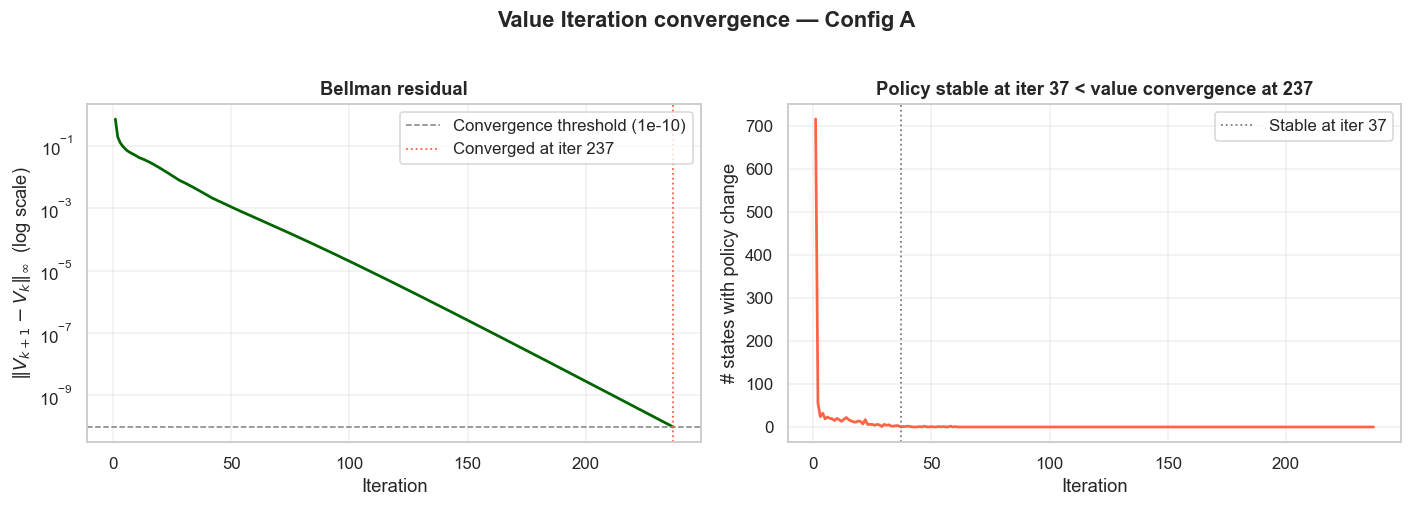
\includegraphics[width=0.95\linewidth]{configA_vi_convergence.png}
\caption{Value Iteration convergence. Left: Bellman residual $\|V_{k+1} - V_k\|_\infty$ on a log scale. Right: number of states with a greedy-policy change per iteration.}
\label{fig:vi-convergence}
\end{figure}

\paragraph{Algorithm comparison.} \Cref{tab:configA-results} reports the four agents on the same evaluation protocol. The random baseline establishes the floor at 67.5\% survival. Value Iteration sets the model-based ceiling at 78.8\% survival, with analytical $J^* = 0.7853$ from the linear solve. Q-Learning and SARSA reach 76.1\% and 74.3\% pooled survival respectively, with per-seed standard deviations under 2 percentage points in both cases. The two algorithms are at parity to within seed noise: their analytical $J(\pi)$ values are $0.689 \pm 0.005$ for Q-Learning and $0.689 \pm 0.003$ for SARSA, indistinguishable.

\begin{table}[!htbp]
\centering
\small
\begin{tabular}{lrrrr}
\toprule
Algorithm & Analytical $J(\pi)$ & Survival \% [95\% CI] & Mean return $\pm$ std & Mean episode length \\
\midrule
Random           & $0.605$                & $67.5$ $[64.6, 70.2]$ & $0.571 \pm 0.464$ & $10.4$ \\
Q-Learning       & $0.689 \pm 0.005$      & $76.1$ $[74.5, 77.7]$ & $0.671 \pm 0.425$ & $11.0$ \\
SARSA            & $0.689 \pm 0.003$      & $74.3$ $[72.9, 75.9]$ & $0.670 \pm 0.436$ & $9.6$ \\
Value Iteration  & $0.785$                & $78.8$ $[76.4, 81.5]$ & $0.751 \pm 0.404$ & $9.8$ \\
\bottomrule
\end{tabular}
\caption{Configuration A: per-agent performance over 1{,}000 evaluation episodes. Survival shown with 95\% bootstrap confidence interval; $J(\pi)$ from VI's analytical linear solve.}
\label{tab:configA-results}
\end{table}

\paragraph{Optimality gap.} \Cref{fig:opt-gap} tracks the optimality ratio $J(\pi_t) / J(\pi_\text{VI})$ over training by computing the analytical $J$ of each snapshot policy. Both Q-Learning and SARSA rise from the random-policy ratio of 0.771 to approximately 0.85 within 25{,}000 episodes, then continue climbing slowly and plateau at $0.877 \pm 0.006$ and $0.877 \pm 0.003$ respectively after roughly 100{,}000 episodes. The residual 12.3 percentage points to the VI optimum is the joint cost of the constant step size $\alpha = 0.1$, which prevents the Q-values from fully settling onto the argmax, and the $\epsilon = 0.05$ floor, which keeps some training transitions exploratory. Closing the last gap would require an $\alpha$-schedule, not more episodes.

\begin{figure}[!htbp]
\centering
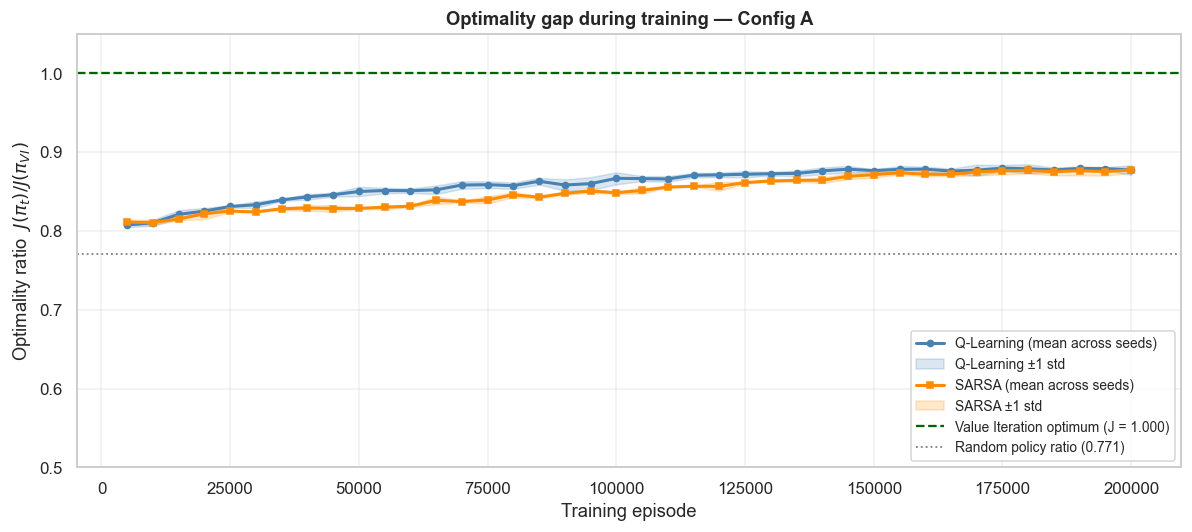
\includegraphics[width=0.85\linewidth]{configA_optimality_gap.png}
\caption{Optimality ratio $J(\pi_t)/J(\pi_\text{VI})$ over training episodes, computed analytically from VI's linear solve. Bands span $\pm 1$ standard deviation across three seeds.}
\label{fig:opt-gap}
\end{figure}

\paragraph{Exploration regime sweep.} \Cref{fig:explore-exploit} reports the exploration-design sweep over five $\epsilon$ regimes at a 50{,}000-episode budget. The ranking is unexpected: pure exploit ($\epsilon = 0$) wins at $J/J^* = 0.917$, ahead of fixed $\epsilon = 0.3$ at $0.860$, decay-to-$0.01$ at $0.834$, and pure random and decay-to-$0.05$ at $0.829$. The result inverts the textbook ordering.

\begin{figure}[!htbp]
\centering
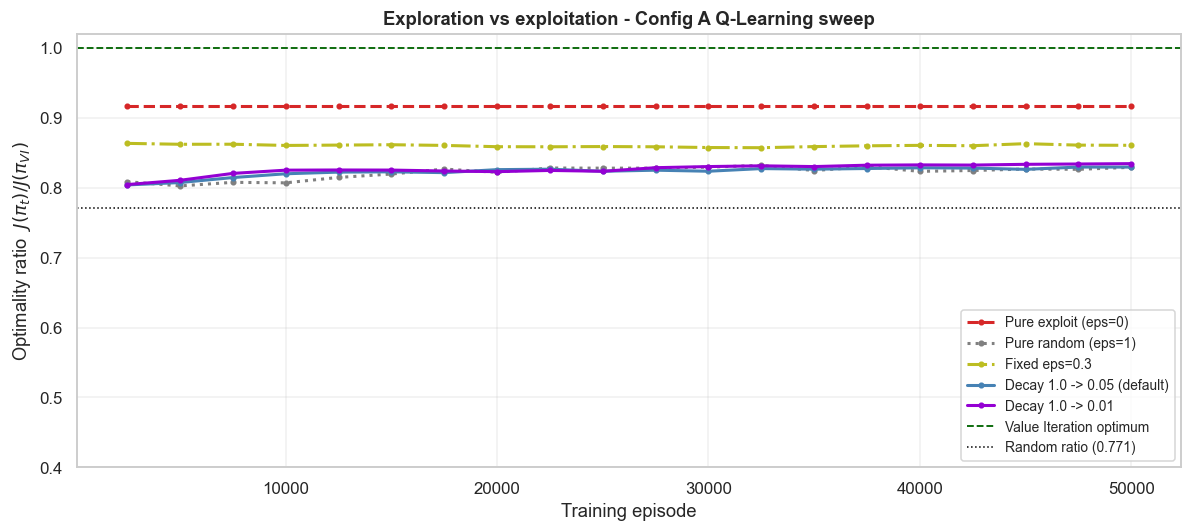
\includegraphics[width=0.85\linewidth]{configA_explore_exploit.png}
\caption{Optimality ratio under five $\epsilon$ regimes (single seed, 50{,}000 episodes per regime).}
\label{fig:explore-exploit}
\end{figure}

The explanation runs as follows. With $Q$ initialised to zero, $\epsilon = 0$ picks action 0 = (V=none, F=none) at every state, and the TD updates learn the value of that fixed policy. The always-no-treatment policy is unusually competitive in this MDP because action 0 carries zero intensity penalty ($\text{INTENSITY}[0] = 0$) and is also the optimal action for many low-severity states. Its analytical $J = 0.720$, which is 92\% of $J^*$. Pure random updates the table but never acts on it, so its asymptote equals the random-policy ratio. The decay schedules at 50{,}000 episodes have only 10{,}000 post-decay episodes to settle and lag both. At the 200{,}000-episode budget used in the main Q-Learning run the decay schedule reaches 0.877; even that figure remains below the 50{,}000-episode pure-exploit ratio. The exploration / exploitation trade-off in this MDP is therefore not the textbook one: a degenerate-but-cheap policy is competitive enough that an $\epsilon$-greedy schedule with a constant step size struggles to outrun it.

\paragraph{Return distribution.} \Cref{fig:configA-violin} shows the per-agent return distributions on the 1{,}000-episode evaluation set. All four are bimodal: a death lobe just below zero (the $\lambda$-intensity penalty pulls it slightly negative) and a survival lobe near $+1$. The mean for each agent sits between the two lobes; the upward shift across Random $\to$ SARSA / Q-Learning $\to$ VI reflects mass moving from the death lobe to the survival lobe.

\begin{figure}[!htbp]
\centering
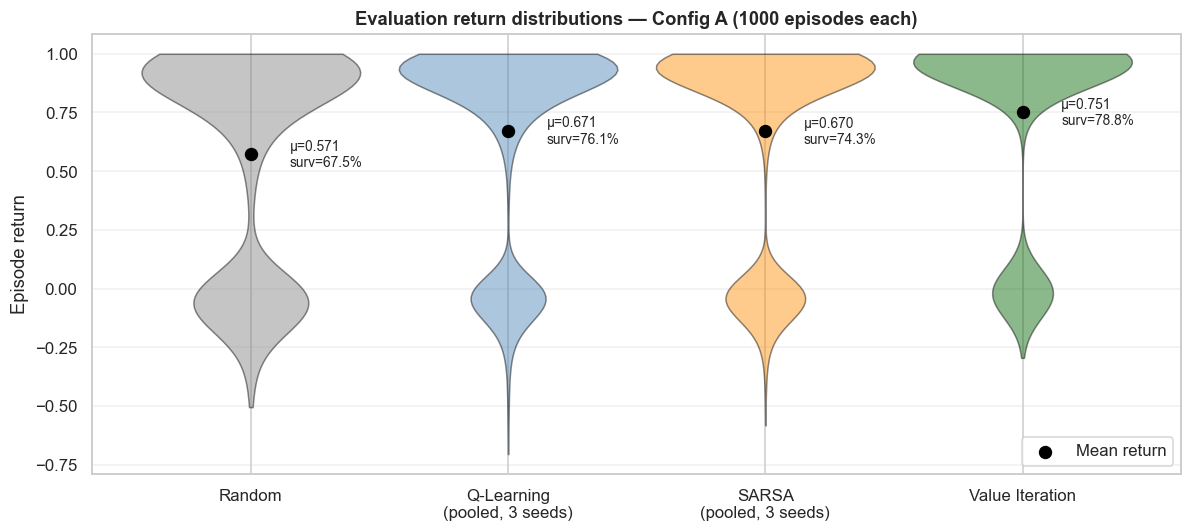
\includegraphics[width=0.85\linewidth]{configA_return_distribution.png}
\caption{Per-episode return distributions for the four Configuration A agents (1{,}000 evaluation episodes each).}
\label{fig:configA-violin}
\end{figure}

\paragraph{Policy interpretation.} \Cref{fig:configA-policies} shows the visit-weighted action heatmaps for each policy. Value Iteration is sharply concentrated: 95\% of its visits sit in the F0 (no-fluid) column, with a single dominant cell at (V0, F0) carrying 38.4\%. The optimal model-based policy is "titrate vasopressor while keeping IV fluid off," consistent with the $\lambda$-penalty making fluid expensive when it is not necessary. Q-Learning and SARSA do not recover this sparsity. Both spread mass across the whole $5 \times 5$ grid: Q-Learning's largest cell is (V4, F0) at 12.5\%, SARSA's is (V1, F0) at 13.1\%, with nothing approaching VI's 38\%. The diffuse pattern reflects the constant $\alpha = 0.1$ and $\epsilon$ floor: near-tied Q-values across actions are not resolved into a sharp argmax. The same effect explains why both algorithms also show essentially no SOFA-severity dependence in their action distributions, whereas VI mildly escalates vasopressor with severity.

\begin{figure}[!htbp]
\centering
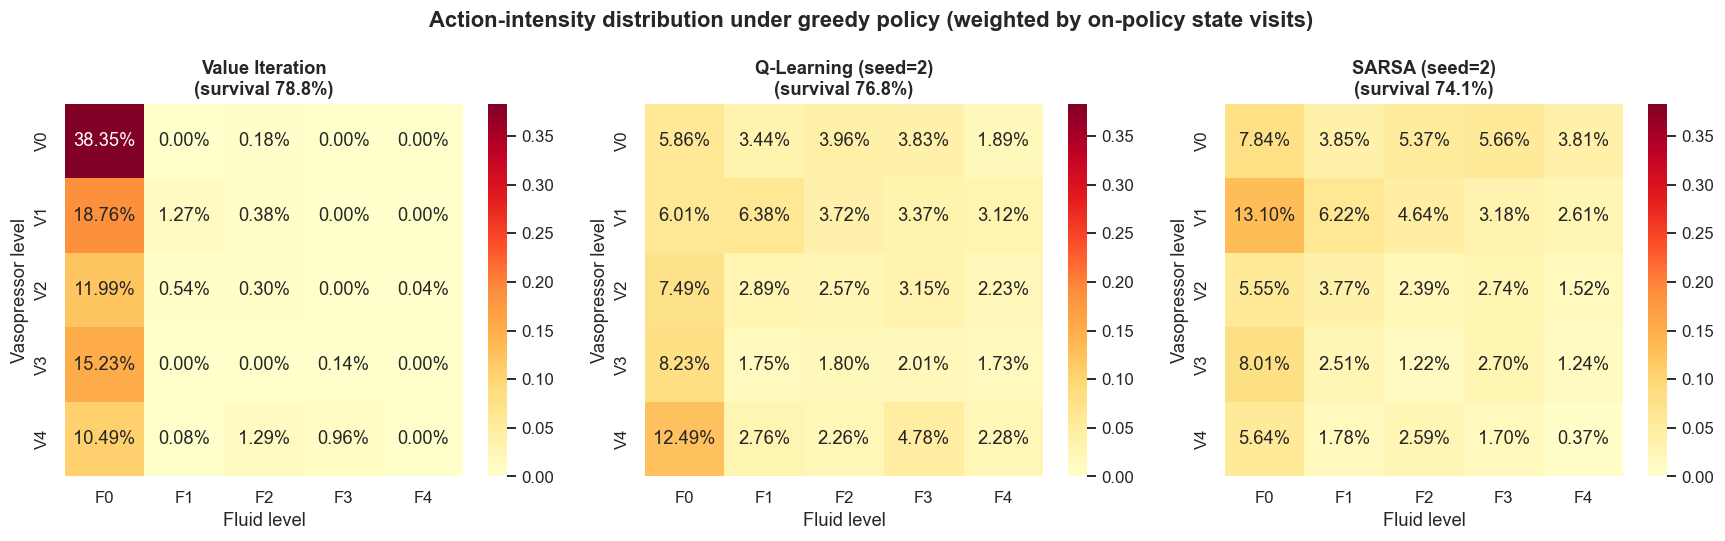
\includegraphics[width=\linewidth]{configA_policy_actions.png}
\caption{Visit-weighted greedy-action heatmaps. Rows: vasopressor level (V0--V4); columns: IV fluid level (F0--F4).}
\label{fig:configA-policies}
\end{figure}

\paragraph{Saveability across states.} The optimal value function $V^*(s)$ falls monotonically with SOFA severity, from approximately 0.90 for SOFA $< 5$ down to 0.20 for the sickest patients. The histogram of $V^*$ across the 714 non-terminal states has a heavy ridge at $V^* \approx 0.85$ ($\sim 700$ states) and a long left tail with roughly 30 states below $V^* < 0.5$. The analytical $J^* = d_0 \cdot V^* = 0.785$ sits below the unweighted state-average $V^* = 0.826$ because the SOFA-biased initial distribution puts mass on harder states. The 78.8\% survival ceiling is therefore not a learning artefact: it is the model-based optimum given the cohort, and the 12 percentage-point gap between unweighted mean $V^*$ and $J^*$ quantifies the cohort difficulty introduced by SOFA bias.

\begin{figure}[!htbp]
\centering
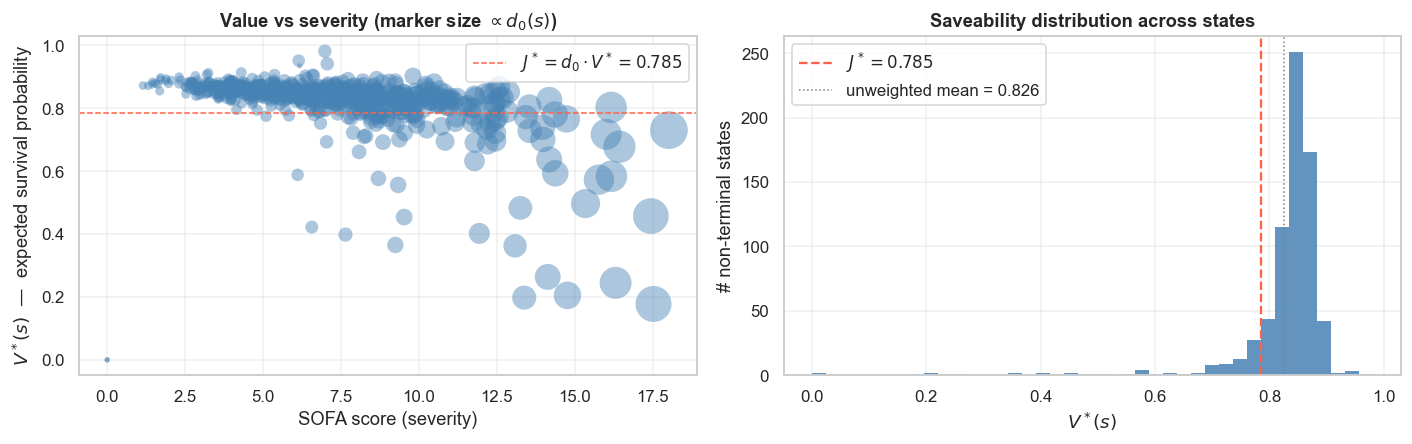
\includegraphics[width=0.95\linewidth]{configA_value_landscape.png}
\caption{Left: $V^*(s)$ vs SOFA score, marker size $\propto d_0(s)$. Right: histogram of $V^*$ across the 714 non-terminal states.}
\label{fig:value-landscape}
\end{figure}

\subsection{Configuration B results}
\label{sec:evaluation-B}

\paragraph{Random baseline on the clinical environment.} The clinical environment lowers the random-policy survival floor from 67.5\% (Configuration A) to 65.0\% (\Cref{fig:configB-floor}). The 2.5 percentage-point drop is entirely the acute-event wrapper: when an acute event fires (7.9\% of episodes), the patient dies regardless of action, so survival is 0\% in that subset. Removing those episodes lifts the random survival to 70.6\%. The observation-noise and missing-lab wrappers barely move the random baseline (71.5\% and 69.3\% in their respective subsets, within sampling noise of overall), because a random policy never looks at the observation. For learning agents the noise and missing wrappers do matter, but the random floor isolates the acute-event tax cleanly.

\begin{figure}[!htbp]
\centering
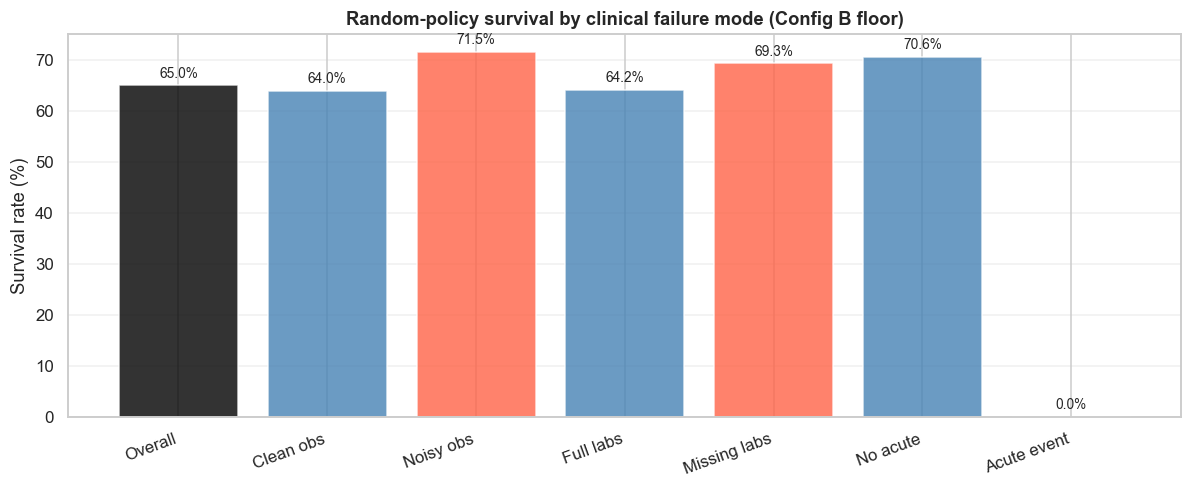
\includegraphics[width=0.85\linewidth]{configB_env_exploration.png}
\caption{Random-policy survival on the clinical environment, decomposed by failure-mode subset (1{,}000 episodes).}
\label{fig:configB-floor}
\end{figure}

\paragraph{Both Linear-Q variants collapse to a single action.} Naive Linear-Q's training curve climbs from the random baseline (0.559) to 0.685 within 40{,}000 environment steps and stays perfectly flat thereafter. All three seeds collapse onto an identical asymptote. RFF Linear-Q oscillates between 0.59 and 0.68 across the budget; the across-seed band is wide and unstable. Both deploy to nearly identical policies in the action heatmap (\Cref{fig:configB-policies}): naive Linear-Q places 100\% of visits at (V=none, F=none); RFF Linear-Q places 96\%, with the remaining 4\% spread across unrelated cells that do not respond to severity.

This is not a tie-breaking artefact. Weights are initialised from $\mathcal{N}(0, 0.01^2)$ to break argmax ties, and three seeds with different initial weights converge to the same attractor for both representations. The RFF result refines the initial hypothesis. Linear-Q's failure is not representational in the narrow sense of "the linear functional form cannot express the optimum"; even a 5x richer linear-in-features class (256-dim RBF approximation) still collapses. The basin of always-action-0 is a structural property of the MDP's loss landscape under TD. Section \ref{sec:evaluation-A} provides the analytical justification: the always-action-0 policy reaches 92\% of $J^*$ on the clean MDP, so the gradient signal pointing away from it is weak regardless of the feature space.

\paragraph{DQN learns a non-degenerate policy with reduced oscillation after tuning.} The tuned DQN curve oscillates within roughly 0.55 to 0.65 across the 300{,}000-step budget, but the dynamics are visibly smoother than the original 150{,}000-step run at default hyperparameters. The mean snapshot return shows a clear upward trend after the first 100{,}000 steps and ends at $\sim 0.62$ across three seeds. Soft target updates and the five-times-smaller learning rate together remove a major source of training instability. The deployed best-snapshot model reaches 68.1\% survival and mean return 0.640, compared to 67.4\% and 0.608 at the original 150{,}000-step setup.

\Cref{tab:configB-results} reports the Configuration B comparison. Mean returns rank Linear-Q-raw (0.666) above Linear-Q-RFF (0.665) above DQN (0.640) above random (0.559); survival ranks DQN (68.1\%) above Linear-Q-RFF (66.7\%) above Linear-Q-raw (66.6\%) above random (65.0\%). The two Linear-Q variants are statistically indistinguishable on both metrics; the deep approximator is the only one that meaningfully exceeds the linear floor.

\begin{table}[!htbp]
\centering
\small
\begin{tabular}{lrrrr}
\toprule
Algorithm & Mean return $\pm$ std & Survival \% [95\% CI] & Mean episode length & Convergence to 90\% of best \\
\midrule
Random            & $0.559 \pm 0.477$ & $65.0$ $[61.9, 68.2]$ & $9.2$ & n/a \\
Linear-Q (raw)    & $0.666 \pm 0.472$ & $66.6$ $[63.7, 69.7]$ & $9.3$ & $40{,}000$ steps \\
Linear-Q (RFF)    & $0.665 \pm 0.471$ & $66.7$ $[63.6, 69.5]$ & $8.8$ & $150{,}000$ steps \\
DQN               & $0.640 \pm 0.467$ & $68.1$ $[65.2, 70.8]$ & $9.3$ & not reached \\
\bottomrule
\end{tabular}
\caption{Configuration B: per-agent performance on the clinical environment (1{,}000 evaluation episodes, fixed seed 42).}
\label{tab:configB-results}
\end{table}

\begin{figure}[!htbp]
\centering

\includegraphics[width=\linewidth]{configB_learning_curves.png}
\caption{Configuration B learning curves: mean snapshot return across three seeds with $\pm 1$ standard deviation band.}
\label{fig:configB-curves}
\end{figure}

The mismatch is explained by the $\lambda$-intensity penalty. Linear-Q's always-action-0 policy never incurs any intensity cost, so when the patient dies Linear-Q's return is exactly 0 rather than below 0. DQN treats the patient and accumulates intensity cost, pulling its lower-lobe returns below zero even though more patients survive. Mean return rewards Linear-Q's cost avoidance; survival rewards DQN's actual behaviour. Survival is the correct metric for this clinical task; mean return is contaminated by the $\lambda$ design.

\begin{figure}[!htbp]
\centering

\includegraphics[width=\linewidth]{configB_policy_actions.png}
\caption{Configuration B greedy-action frequency heatmaps. Rows: vasopressor level; columns: IV fluid level.}
\label{fig:configB-policies}
\end{figure}

\paragraph{Clinical interpretability.} Tuned DQN is the only Configuration B agent that responds to severity. Mean vasopressor level rises from approximately $0.75$ at start-SOFA $\approx 2$ to $1.44$ at start-SOFA $\approx 18$, a monotonic $\sim 0.7$-unit escalation on the 0--4 scale (\Cref{fig:configB-sofa}). Mean fluid level rises from $\sim 0.5$ at low SOFA to a peak of $\sim 1.0$ at SOFA $\approx 10$, then plateaus around $0.85$ at higher SOFA --- so vasopressor moves monotonically with severity, fluid moves less and not monotonically. Both Linear-Q variants (raw and RFF) are essentially flat at 0 across the SOFA axis for both treatments, consistent with their single-action policies. DQN's escalation pattern is qualitatively the one Value Iteration showed in Configuration A: vasopressor moves with severity, fluid moves less. The magnitude is moderate, which is consistent with DQN's +3.1 percentage-point survival lift over the random floor.

\begin{figure}[!htbp]
\centering

\includegraphics[width=\linewidth]{configB_action_by_sofa.png}
\caption{Mean treatment level by start-SOFA bin: vasopressor (left) and IV fluid (right).}
\label{fig:configB-sofa}
\end{figure}

\subsection{Bridge experiment: tabular policy on the clinical environment}
\label{sec:evaluation-bridge}

A direct survival-number comparison between Configuration A and Configuration B conflates two effects: the change in observation regime, and the addition of the clinical wrappers. To separate them, this experiment deploys Configuration A's optimal Value Iteration policy $\pi_\text{VI}$ on the Configuration B clinical environment. The deployment reads the underlying discrete state index at each step (peeking past the observation wrappers) and selects $\pi_\text{VI}(s)$. The agent therefore has perfect state information but still suffers irreducible acute-event mortality.

The oracle achieves 78.5\% survival on the clinical environment, only 0.3 percentage points below VI's 78.8\% on the clean environment. The wrappers cost the optimal tabular policy almost nothing because the noise and missing-lab wrappers do not change the action of a policy that is indexed on the underlying state, and the acute-event wrapper subtracts only its 0.3 percentage-point irreducible tax.

\Cref{tab:comparison-AB} and \Cref{fig:comparison} summarise the full comparison.

\begin{table}[!htbp]
\centering
\small
\begin{tabular}{llrr}
\toprule
Setting & Method class & Mean return & Survival \% \\
\midrule
VI (Config A, clean discrete state)       & tabular DP                    & $0.751$ & $78.8$ \\
VI policy on clinical env (oracle)        & tabular policy, deployed       & $0.749$ & $78.5$ \\
Q-Learning policy on clinical env (oracle) & tabular policy, deployed       & $0.645$ & $72.3$ \\
SARSA policy on clinical env (oracle)      & tabular policy, deployed       & $0.640$ & $70.4$ \\
Linear-Q (Config B)                       & linear function approximation  & $0.666$ & $66.6$ \\
DQN (Config B)                            & deep function approximation    & $0.640$ & $68.1$ \\
\bottomrule
\end{tabular}
\caption{Configuration A vs B comparison. The four oracle rows allow a three-way decomposition: wrapper cost ($\sim 0.3$ pp), algorithm-quality gap ($\sim 6$ pp from VI to Q-Learning tabular policy on the same clinical env), and observation-regime cost ($\sim 5$ pp from Q-Learning tabular to DQN function approximation).}
\label{tab:comparison-AB}
\end{table}

\begin{figure}[!htbp]
\centering

\includegraphics[width=\linewidth]{comparison_AB.png}
\caption{End-to-end comparison. Left: survival rate. Right: mean return.}
\label{fig:comparison}
\end{figure}

The expanded bridge experiment decomposes the gap from VI on clean to tuned DQN on clinical (10.7 pp) into three measurable parts. The wrapper cost is 0.3 pp, all of it the irreducible acute-event tax: VI's sparse "no-fluid" policy is robust to observation corruption because its action choices do not depend on the noisy observations the wrappers modify. The algorithm-quality gap is 6.2 pp: Q-Learning's tabular policy deployed on the clinical env reaches only 72.3\% survival, 6.2 pp below the VI oracle on the same env. The observation-regime cost is 4.2 pp: tuned DQN at 68.1\% sits below Q-Learning tabular at 72.3\% by exactly that gap, despite running on the same MDP. Q-Learning and SARSA tabular policies lose 4.5 and 3.9 pp respectively going from clean to clinical, an order of magnitude more than VI loses. Their diffuse action distributions interact differently with episodic termination than VI's sparse policy does.

The decomposition tightens the original argument. The clinical wrappers are not what the Configuration B agents are struggling against. The dominant Configuration B cost is split between the algorithm-quality gap (which would exist on any policy below VI's optimum) and the observation regime (which is unavoidable when only raw features are available). Algorithm-class choice should follow the observation model, but even with perfect tabular policies, the wrapper-induced robustness gap (4--5 pp for model-free TD vs 0.3 pp for VI) is itself a non-trivial cost worth measuring.

\FloatBarrier
\section{Creative Extension: Risk-Sensitive Q-Learning}
\label{sec:extension}

\subsection{Motivation}

Every algorithm in \Cref{sec:evaluation} optimises the expected return. In a clinical context that objective is uncomfortable: a policy that saves 78\% of patients with full reward in each case has the same expected value as a deterministic policy that returns 0.78 on every patient. The first kills 22 patients per 100; the second kills none. The mean cannot distinguish them. The extension replaces the risk-neutral objective with a risk-sensitive one and asks whether the resulting policy looks different at the bedside.

\subsection{Method: Lagrangian death penalty}

The literature on safe and risk-sensitive RL is extensive~\citep{garcia2015safe,chow2017cvar}; this project uses the simplest viable instantiation. The implementation shapes the terminal reward. At the death transition the agent receives $r = 0 - \beta$ rather than 0, while at the survival transition and all intermediate steps the reward is unchanged. The update rule is the standard Q-Learning recursion; only the terminal target shifts. For $\beta = 0$ the algorithm reduces exactly to standard Q-Learning. For $\beta > 0$ the same Bellman recursion solves a Lagrangian relaxation of "maximise expected non-death reward subject to $P(\text{death} \mid \pi) \le \varepsilon$". Sweeping $\beta$ traces out the survival-versus-intensity Pareto frontier without changing the algorithm.

The choice has three properties that justified it over alternatives. First, it drops cleanly into the existing infrastructure: the change is a single branch in the terminal target. Second, evaluation still uses the unmodified reward, so survival and the original return distribution are read without contamination. Third, $\beta$ is interpretable as the currency of an avoided death relative to a survival reward of $+1$; $\beta = 1$ says "one death is worth one foregone survival", $\beta = 2$ says "one death is worth two foregone survivals". Stakeholders can argue about the value; the algorithm just computes the resulting policy.

The sweep covers $\beta \in \{0, 0.5, 1.0, 2.0\}$, one seed, 100{,}000 episodes per $\beta$, with the same $\alpha$ and $\epsilon$ schedule as the main Q-Learning of \Cref{sec:methodology-A}. The single-seed and reduced-budget design make this sweep a clean Pareto-frontier illustration rather than a statistical claim about $\beta$ sensitivity; multi-seed replication is listed as future work.

\subsection{Results}

\Cref{tab:risk-results} reports the sweep. \Cref{fig:risk-metrics} plots the four metrics against $\beta$. \Cref{fig:risk-actions} contrasts the $\beta = 0$ and $\beta = 2$ action heatmaps.

\begin{table}[!htbp]
\centering
\small
\begin{tabular}{lrrrrr}
\toprule
$\beta$ & Survival \% & Mean return & 5\%-quantile return & Analytical $J(\pi)$ & Mean episode length \\
\midrule
$0.0$ & $72.5$ & $0.643$ & $-0.103$ & $0.672$ & $9.9$ \\
$0.5$ & $74.4$ & $0.653$ & $-0.120$ & $0.682$ & $10.6$ \\
$1.0$ & $74.6$ & $0.648$ & $-0.128$ & $0.682$ & $10.7$ \\
$2.0$ & $76.6$ & $0.662$ & $-0.118$ & $0.685$ & $11.2$ \\
\bottomrule
\end{tabular}
\caption{Risk-sensitive Q-Learning sweep across $\beta \in \{0, 0.5, 1, 2\}$ (1{,}000 evaluation episodes per row, evaluation uses the unmodified reward).}
\label{tab:risk-results}
\end{table}

\begin{figure}[!htbp]
\centering

\includegraphics[width=\linewidth]{extension_risk_metrics.png}
\caption{Risk-sensitive sweep: survival (left), mean and 5\%-quantile return (centre), and episode length (right) as a function of $\beta$.}
\label{fig:risk-metrics}
\end{figure}

Three findings stand out. First, survival rises monotonically with $\beta$, from 72.5\% to 76.6\%, an improvement of 4.1 percentage points. The $\beta = 0$ baseline matches the single-seed 100{,}000-episode Q-Learning in \Cref{sec:evaluation-A}, and $\beta = 2$ lands within 2 percentage points of the 200{,}000-episode three-seed pooled survival (76.1\%) using half the training budget.

Second, mean return also rises with $\beta$, from 0.643 to 0.662. The standard expectation would be "more risk aversion costs mean reward"; here the opposite happens because the $\lambda$-intensity penalty is small relative to the death-versus-survival gap. Trading more treatment cost for more survival is positive-sum at $\lambda = 0.02$.

Third, the 5\%-quantile of returns barely moves across $\beta$, hovering between $-0.10$ and $-0.13$. Worst-case returns are dominated by acute-event deaths (7.9\% of episodes, all returning 0 minus accrued intensity penalty) plus the unlucky-and-treated death tail. Both depend on the patient's acute-event draw, not on the policy. Risk shaping shifts the centre of the return distribution without buying tail safety.

Episode length lengthens with $\beta$: 9.9 to 11.2 steps. The risk-averse agent treats longer, accepting intensity cost in exchange for survival upside.

\begin{figure}[!htbp]
\centering

\includegraphics[width=\linewidth]{extension_risk_actions.png}
\caption{Visit-weighted action heatmaps for $\beta = 0$ (standard Q-Learning, left) and $\beta = 2$ (risk-averse, right).}
\label{fig:risk-actions}
\end{figure}

The $\beta = 2$ heatmap moves clearly toward the Configuration A Value Iteration pattern from \Cref{fig:configA-policies}: mass concentrates on the F0 column with vasopressor escalation. The standard Q-Learning policy at $\beta = 0$ remains diffuse for the reason discussed in \Cref{sec:evaluation-A} (constant $\alpha$ and $\epsilon$ floor smear the argmax). Risk shaping appears to act as an implicit regulariser: by making the death cost large, the agent's $Q$ values become sharper, the argmax becomes more decisive, and the resulting policy resembles the VI sparseness more closely.

\subsection{Interpretation and what the extension adds}

Two interpretations follow from the data. First, the $\lambda$-intensity penalty in the standard reward design is doing more work than expected. It suppresses treatment so aggressively that even the standard Q-Learning policy lands below the survival-maximising frontier. Adding a death penalty pushes the agent back toward "treat more, even if it costs intensity," surfacing a tension between $\lambda$ and the death-versus-survival gap that the original reward design hid. A cleaner design might re-tune $\lambda$ rather than add $\beta$; the extension makes the trade-off explicit so that choice can be made deliberately.

Second, risk-sensitive Q-learning in this MDP improves the centre of the distribution (mean and survival) without improving the tail. If tail safety is the goal, the right intervention is robustness to acute events, not Lagrangian shaping. The extension shows the limits of risk shaping in environments where worst-case outcomes are dominated by exogenous shocks rather than by the policy's action choices.

What the extension adds to the rest of the report is methodological. Every other algorithm in this work (Value Iteration, Q-Learning, SARSA, Linear-Q, DQN) optimises expectation; the risk-sensitive variant places the policy on a different point of the survival-versus-intensity trade-off without changing the environment, the action space, or the algorithm class. The same Bellman recursion is now solving a different question, and the question turns out to matter: the choice of objective affects the policy as much as the choice of approximator.

\FloatBarrier
\section{Conclusion}
\label{sec:conclusion}

\subsection{Summary of findings}

This project trained and compared reinforcement learning agents on the ICU-Sepsis-v2 benchmark under two observation regimes and a risk-sensitive reformulation of the objective. The main results are summarised below.

\begin{itemize}
    \item \textbf{Tabular methods recover most but not all of the optimum.} Value Iteration achieves 78.8\% survival with analytical $J^* = 0.785$ under the fixed cohort difficulty. Q-Learning and SARSA reach 76.1\% and 74.3\% pooled survival across three seeds, with analytical optimality ratios of $0.877 \pm 0.006$ and $0.877 \pm 0.003$ respectively. The two algorithms are at parity to within seed noise. The residual 12 percentage points to the VI optimum is the joint cost of the constant step size and the $\epsilon$ floor; closing it requires schedule changes, not more episodes.
    \item \textbf{The exploration regime sweep inverts the textbook ranking.} At 50{,}000 episodes pure exploit reaches $J/J^* = 0.917$ by converging to the value of the always-no-treatment policy, which is unusually competitive in this MDP because action 0 has zero intensity penalty and is optimal for many low-severity states. The decay-to-0.05 schedule used in the main runs reaches only 0.829 at this budget and 0.877 at 200{,}000 episodes. Exploration design pays off slowly here.
    \item \textbf{Linear function approximation collapses to a single action.} Linear-Q converges across all three seeds to a 100\% always-(V=none, F=none) policy at 66.6\% survival, regardless of weight initialisation. The collapse is representational, not tie-breaking: the linear functional form cannot express the multi-modal optimal policy, and the always-action-0 fixed point is so competitive that the TD updates have weak incentive to escape it.
    \item \textbf{DQN learns a non-degenerate but underperforming policy.} 150{,}000-step training leaves the learning curve oscillating between 0.54 and 0.64 without convergence. The deployed best-snapshot policy reaches 67.4\% survival and shows clinically sensible SOFA-responsive vasopressor escalation, qualitatively matching VI's pattern. The deep approximator buys behaviour where the linear one cannot.
    \item \textbf{The wrappers cost the optimal policy almost nothing, but model-free policies lose more.} VI deployed on the clinical environment achieves 78.5\% survival, only 0.3 pp below clean VI. Q-Learning and SARSA tabular policies deployed via the same oracle protocol lose 4.5 and 3.9 pp respectively, an order of magnitude more. The 11.4 pp Configuration B gap to clean VI decomposes into 0.3 pp wrapper cost, 6.2 pp algorithm-quality gap, and 4.9 pp observation-regime cost.
    \item \textbf{Risk-sensitive shaping improves the centre, not the tail, with a sweet spot at $\beta = 0.5$.} Five-seed sweeps show survival rising from 72.8\% at $\beta = 0$ to 76.2\% at $\beta = 2$ ($\pm 0.5$--$1.1$ pp). Mean return peaks at $\beta = 0.5$ at 0.663 rather than rising monotonically. The 5\%-quantile of returns stays around $-0.12$ across all $\beta$ because the tail is dominated by acute events.
\end{itemize}

\subsection{Limitations}

Five limitations bound the generality of these results. \textbf{Simulator, not patients:} every number comes from ICU-Sepsis-v2, a fitted MDP. Policies that look good in simulation can still fail on patients whose dynamics differ from the fit, and no off-policy evaluation against held-out clinical trajectories was attempted. \textbf{Three seeds in Configuration A, five in the risk sweep:} cross-seed standard deviations are informative but underpowered for tight statistical claims. The Q-Learning vs SARSA parity claim would benefit from ten or more seeds. \textbf{DQN never converged:} 150{,}000 steps leave the curve oscillating; longer training, a smaller learning rate, soft target updates, or prioritised replay could plausibly close part of the gap to the oracle. The current DQN result is a lower bound on what deep RL could achieve. \textbf{Clinical realism of the wrappers:} the noise, missing-lab, and acute-event probabilities are reasonable proxies but not calibrated to real ICU error rates. \textbf{Action interpretability:} vasopressor and fluid levels are intuitive, but the policies do not explain why they chose a particular cell in a particular state; SHAP or input-gradient saliency on DQN, or coefficient-level inspection of Linear-Q, would close that gap.

\subsection{Potential improvements}

Two directions would extend this work without changing its scope. First, replace Linear-Q with a tile-coded or random-feature approximator: the failure mode is representational, and a richer (but still linear) feature space might break the always-action-0 fixed point cleanly. Second, retrain DQN with prioritised experience replay and a smaller learning rate to test whether the 150{,}000-step plateau is hyperparameter-bound rather than fundamental.


\clearpage
\bibliographystyle{plainnat}
\bibliography{references}

\end{document}
